\documentclass{beamer}
\usetheme{Warsaw}
\setbeamertemplate{headline}{}
\graphicspath{ {./images/} }
\usepackage{amsmath}

\usepackage{amssymb}
\usepackage{algpseudocode}
\usepackage{algorithm}
\usepackage{setspace}
\usepackage{graphicx}
\graphicspath{ {./images/} }
\usepackage{hyperref}
\usepackage{siunitx}
\usepackage{amsmath}
\usepackage{caption}
\usepackage{subcaption}

\title[Binding affinity prediction of PL complexes using ML]{Binding Affinity Prediction of Protein-Ligand complexes using Machine Learning}

\author[Abdus Salam Khazi]
{
    \textbf{MSc Project}\\
    Abdus Salam Khazi
}

\institute{Supervisors: \\
            \begin{tabular}{ll}
		    	Simon Bray \& Alireza Khanteymoori
		    \end{tabular}
}

\date{\today}
\logo{
\includegraphics[width=.2\textwidth]{Logo}}

\hypersetup{
    colorlinks=false,
    linkcolor=blue,
    filecolor=magenta,      
    urlcolor=cyan,
}

\begin{document}

\begin{frame}
\titlepage
\end{frame}

\begin{frame}{Table of Contents}
\tableofcontents
\end{frame}

\section{Introduction: Biological Background}

\begin{frame}[t]{Biological Background}
What are proteins and ligands? 
\begin{itemize}
\item \textbf{Proteins:} Complex molecules that are work-horses (machines) of a living organism.
\item \textbf{Ligands:} Molecules that bind to (receptor) proteins.

\item Proteins and ligands bind together to form protein-ligand complexes.

\end{itemize}

\begin{figure}[htb]
  \centering
    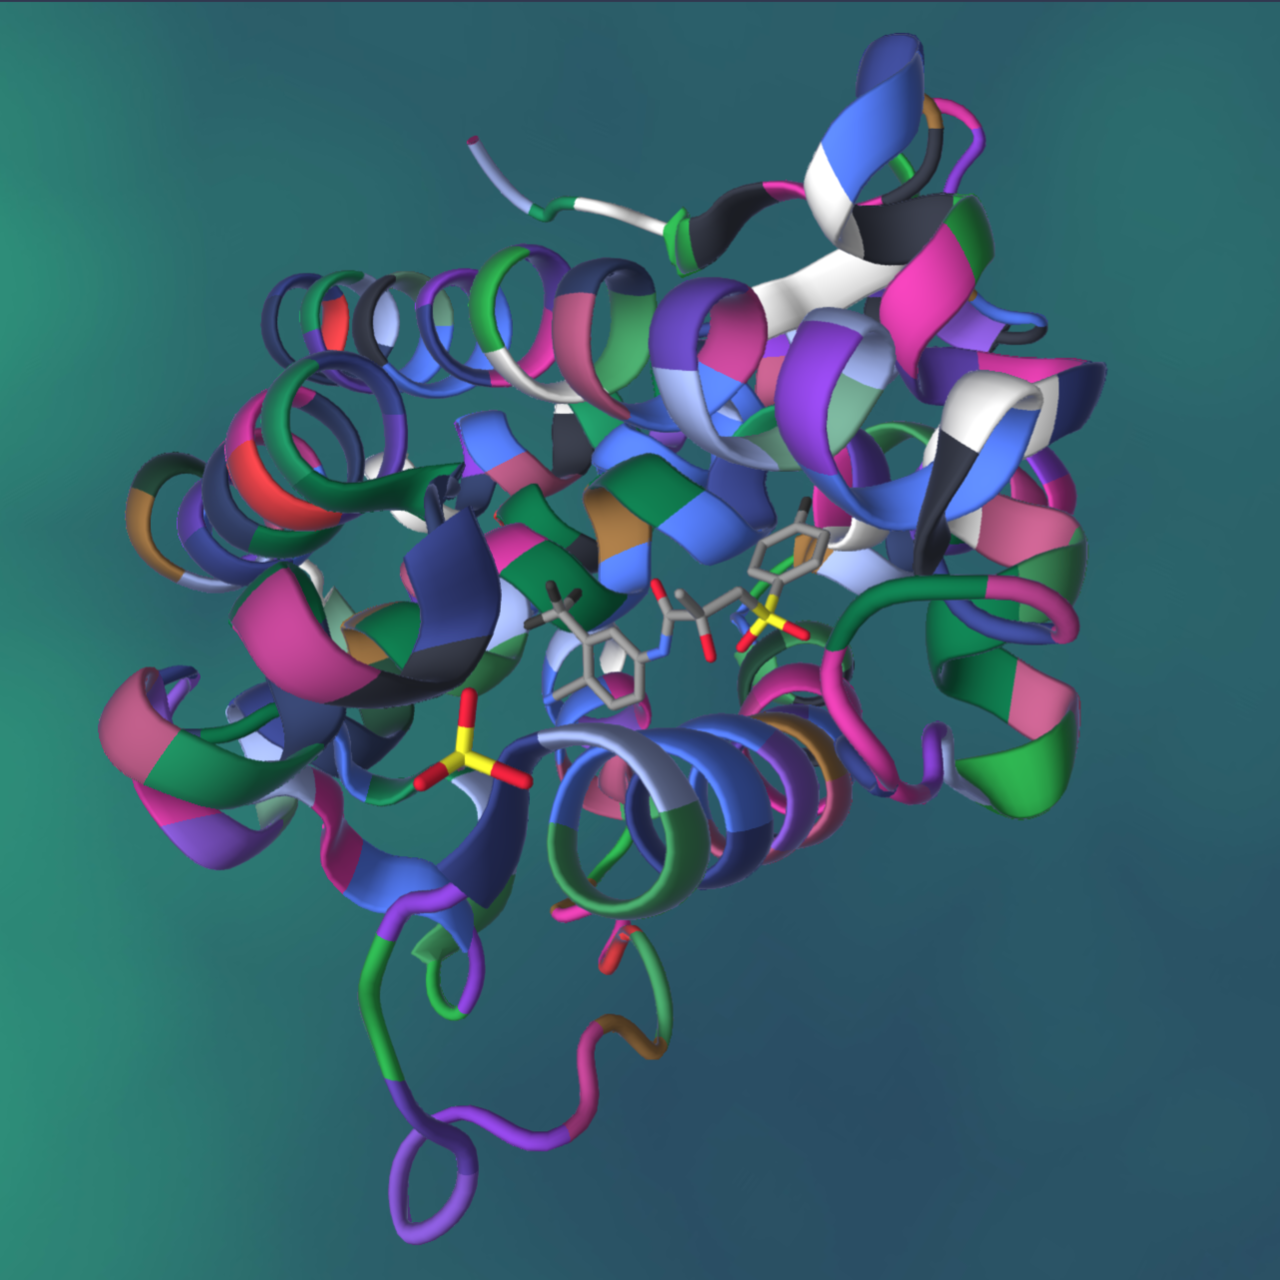
\includegraphics[scale=0.07]{images/pl_complex}
    \caption{Haemoglobin transporter protein.}
    \label{fig:HaemoglobinTransporterImage}
\end{figure}

\end{frame}

\begin{frame}[t]{Biological Background}
\textbf{Protein-Ligand complexes}

\begin{itemize}
\item Ligands bind to proteins at "cavity" like locations called pockets.
\item The pockets and the ligands are complementary in shape.
\end{itemize}

\textbf{Drugs}
\begin{itemize}
\item Drugs are ligand molecules that bind to proteins.
\item They cause a therapeutic effect after binding to the proteins.
\end{itemize}

\begin{figure}[htb]
  \centering
    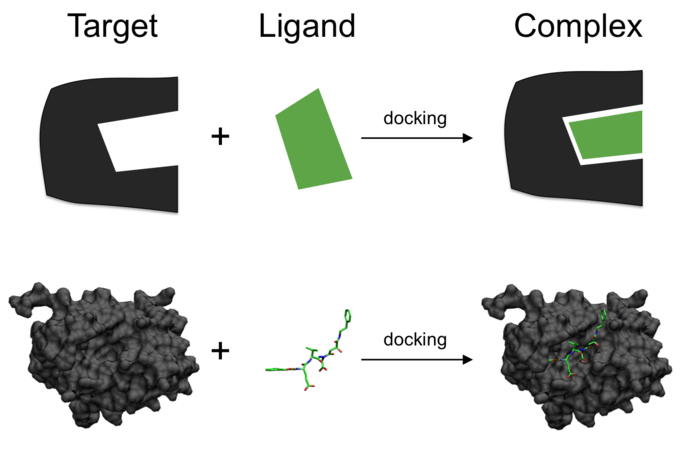
\includegraphics[scale=0.45]{images/lock_and_key}
    \caption{Lock and Key hypothesis in molecular docking.}
    \label{fig:lockandkey}
\end{figure}


\end{frame}

\begin{frame}[t]{Biological Background}
Protein-Binding Affinity

\begin{itemize}
\item Assume a dynamic system in which protein $P$ and ligand $L$ are binding and unbinding continuously.
\item Binding affinity can be quantified by using disassociation constant $k_d$ (\textbf{at equilibrium}).
$$ k_d = \frac{[P][L]}{[PL]}$$
\end{itemize}

Here $[P] = $ Protein concentration, $[L] = $ Ligand concentration and $[PL] = $ Protein-Ligand complex concentration.

\end{frame}

\section{Problem Definition}

\begin{frame}[t]{Problem Definition}

\begin{itemize}
\item Determining if a potential drug (ligand) can bind to a target protein is very expensive \cite{drugdiscoverycost}.
\item The project tries to reduce the drug discovery costs by eliminating bad leads.
\item \textbf{Problem definition}: Predict protein-ligand binding affinity using "In-Silico" methods. 
\end{itemize}

\begin{figure}[htb]
  \centering
    \includegraphics[scale=0.4]{images/ProjectOverview}
    \caption{Project Overview}
    \label{fig:ProjectOverviewImage}
\end{figure}

\end{frame}

\begin{frame}[t]{Problem Definition}
There are various problems in the protein-ligand domain.  The following figure shows the classification tree.

\begin{figure}[htb]
  \centering
    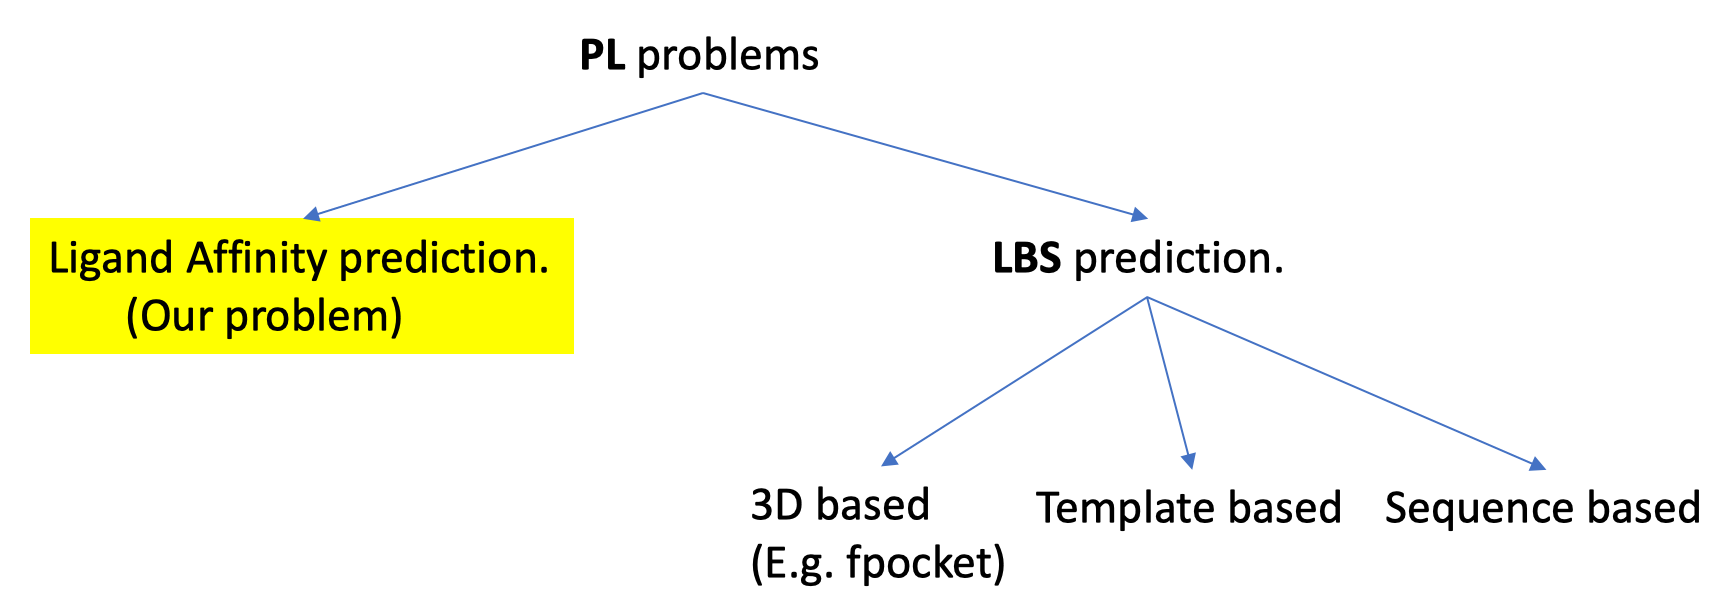
\includegraphics[scale=0.35]{images/pl_problem_classification}
    \caption{Protein-Ligand problem classification.}
    \label{fig:plproblemclassification}
\end{figure}

\end{frame}

\section{Data Processing and Analysis}

\begin{frame}[t]{Feature Extraction}

\begin{itemize}
\item The input data to the ML model is extracted from a database called PDB Data bank.
\item \textit{fpocket} and \textit{RDKit} were used to extract the features of proteins and ligands.
\item The input features contain information about the 3D structures of the proteins and the ligands.
\item Protein Features (55) + Ligand Features (402) = 457 features
\end{itemize}

\begin{figure}[htb]
  \centering
    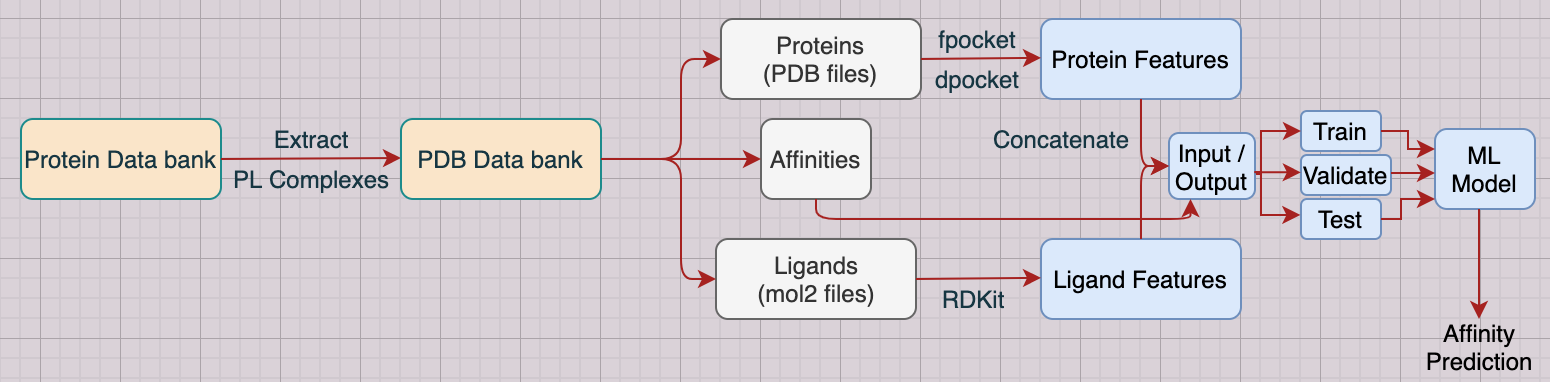
\includegraphics[scale=0.36]{images/DataInputOverview}
    \caption{Data Input Overview.}
    \label{fig:projectoverviewimage}
\end{figure}


\end{frame}

\begin{frame}[t]{Data Preprocessing}
\begin{itemize}
\item Data points containing NaN (Not a number) values were removed from the data.
\item PCA (Principal Component Analysis) was used to find the variance contribution of the features.
\item Feature \textit{IPC} was log scaled for numerical safety during training.
\end{itemize}

\begin{figure}
     \centering
     \begin{subfigure}[b]{0.4\textwidth}
         \centering
    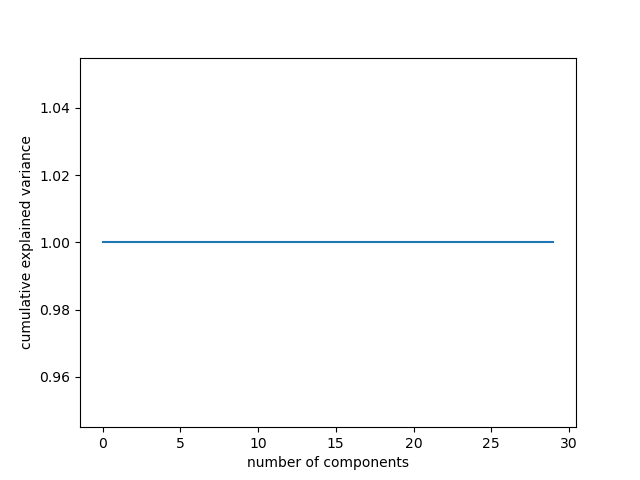
\includegraphics[scale=0.25]{images/pcaligandanalysisIPC}
    \caption{With original Ligand feature IPC.}
    \label{fig:pcaproteinanalysisIPC}
     \end{subfigure}
     \hfill
     \begin{subfigure}[b]{0.4\textwidth}
         \centering
        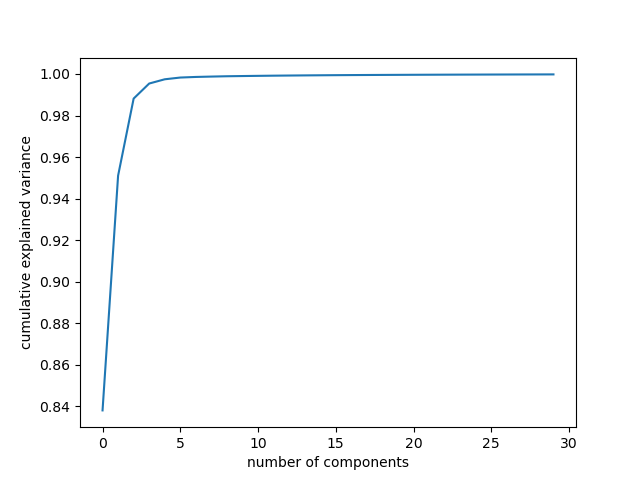
\includegraphics[scale=0.25]{images/pcawithscaledIPC}
        \caption{With log scaled Ligand feature IPC.}
        \label{fig:pcawithscaledIPC}
     \end{subfigure}
     \caption{Cumulative PCA of ligand features.}
     \label{fig:PCAAnalysis}
\end{figure}

\end{frame}

\begin{frame}[t]{Feature Selection}
Feature selection strategies:
\begin{itemize}
\item \textbf{Manual:} 121 ligand descriptors given by domain expert + all protein descriptors.
\item \textbf{Output Correlation}: Features with the best \textit{Pearson} or \textit{Spearman} correlation w.r.t the affinity score (output) were selected.
\item \textbf{Genetic Algorithms}:  \cite{geneticalgorithmsresearchpaper}
\begin{itemize}
\item Each chromosome is represented by $\mathbf{B}^{457}$.  (E.g $[1100..10..]$)
\item $\mathrm{Chromosome Score} = \mathrm{Model}\_\mathbf{R2}_{score} * \textrm{Features Eliminated}$
\end{itemize}

\begin{figure}[htb]
  \centering
    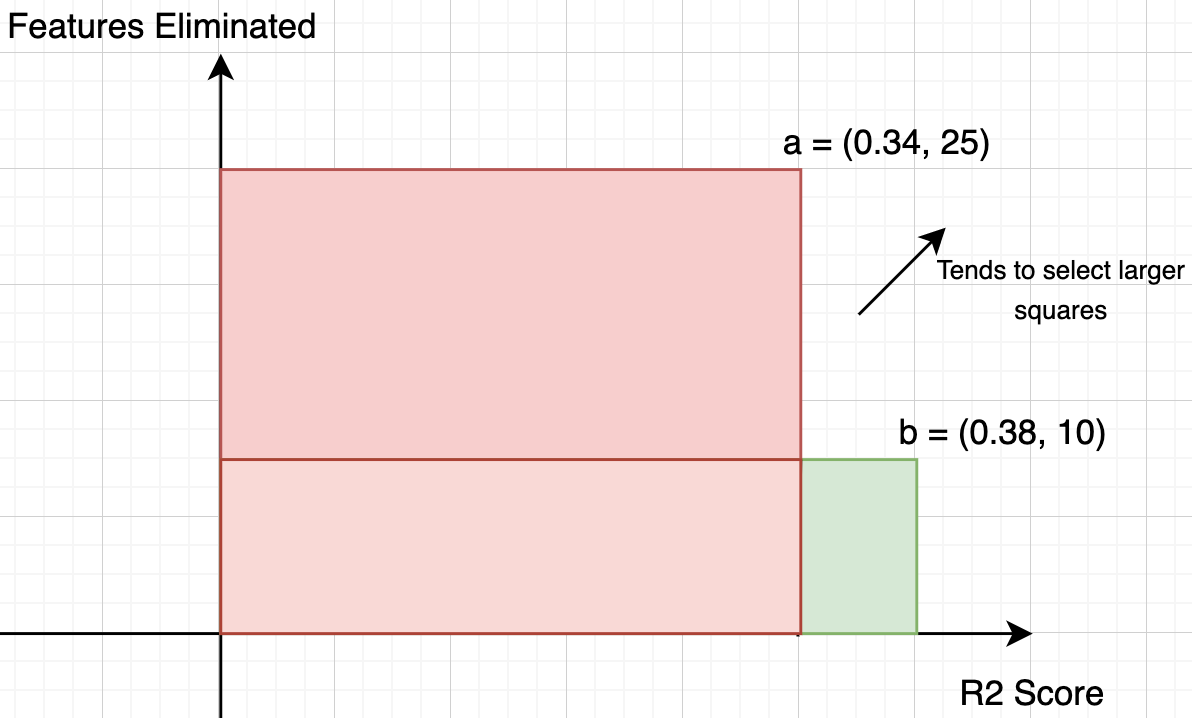
\includegraphics[scale=0.25]{images/scoreFuntionMultiObject}
    \caption{Genetic Algorithm score function representation.}
    \label{fig:scorefunctionfigure}
\end{figure}

\end{itemize} 

\end{frame}

\begin{frame}[t]{Dealing with measurement resolution}
\begin{itemize}
\item Each complex has a measurement resolution (\si{\angstrom} units).
\item Data quality (3D image detail) $\propto \frac{1}{\mathrm{Measurement
Resolution}}$
\item The weighting of the data point was done by
\begin{itemize}
\item Hyperbolic Weighting: $ W_\mathrm{Hyperbolic} = \frac{ \mathrm{\max{R_{1 ...  n}}}}{R_i}$
\item Linear Weighting: $W_\mathrm{Linear}  = (\mathrm{\max{R_{1 ...  n}}} + 1) - R_i$
\end{itemize} 
\end{itemize}

\begin{figure}
     \centering
         \centering
    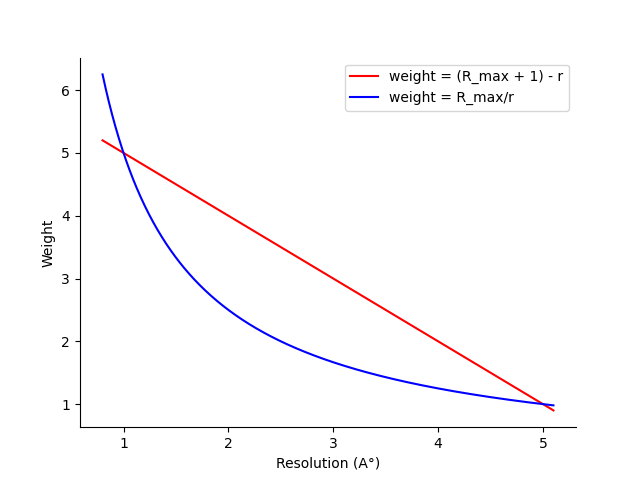
\includegraphics[scale=0.40]{images/graphingformula}
    \caption{Weight calculation formulae.}
    \label{fig:graphingformula}
\end{figure}

\end{frame}


\begin{frame}[t]{Feature Family Correlations}
\begin{itemize}
\item Features can be divided into families.
\item Within some families, the features are correlated.
\item ML models need to take into account this issue.
\end{itemize}
\begin{figure}[htb]
    \begin{subfigure}[b]{0.49\textwidth}
         \centering
         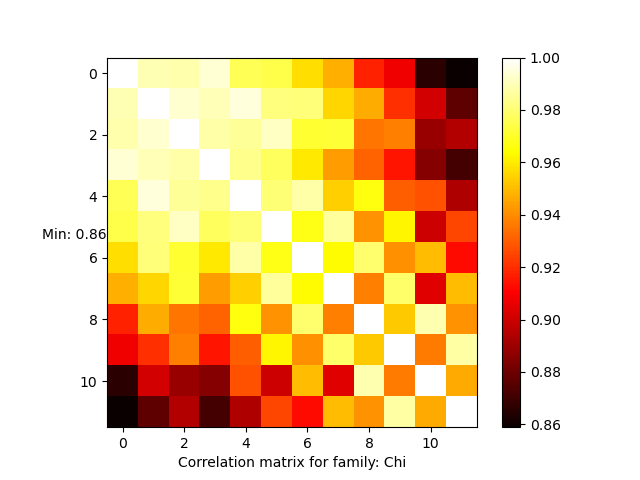
\includegraphics[scale=0.25]{images/correlationChi}
        \label{fig:correlationChi}
     \end{subfigure}
     \hfill
    \begin{subfigure}[b]{0.49\textwidth}
         \centering
         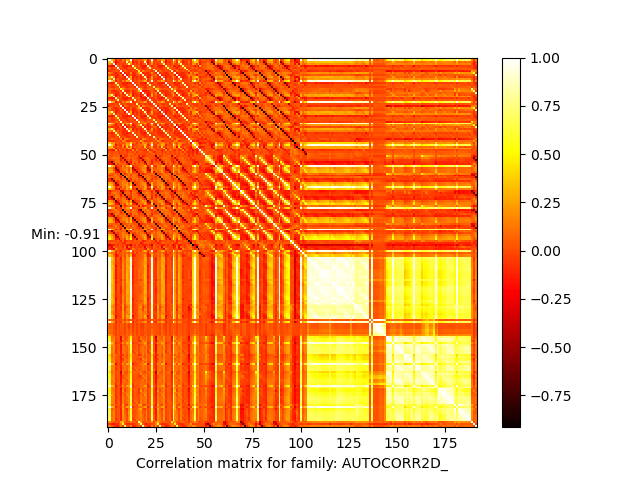
\includegraphics[scale=0.25]{images/correlationAUTOCORR2D}
        \label{fig:correlationfr}
     \end{subfigure}
     \caption{Correlation Heat Map of families: Chi (left) and AUTOCORR2d\_ (right).}
     \label{fig:correlationheatmap}
\end{figure}
\end{frame}


\section{Testing strategy}

\begin{frame}[t]{Testing strategy}
\textbf{Reproducibilty}:
\begin{itemize}
\item \textbf{Random Seed} (Execution ID) reported for every execution.
\end{itemize}

\textbf{Result quality analysis}:
\begin{itemize}
\item $\mathbf{R}^2$ \textbf{score} (\textit{Coefficient of determination}): $R^2  \in (- \infty, 1.0]$ where $1.0$ is the best score. 
\item \textbf{Visualization:}
The model's prediction is visualized as a 2D scatter plot. 
The best plot is $y = x$ line which corresponds to the best $R^2$ score of 1.0.

\end{itemize}

\begin{figure}[htb]
  \centering
    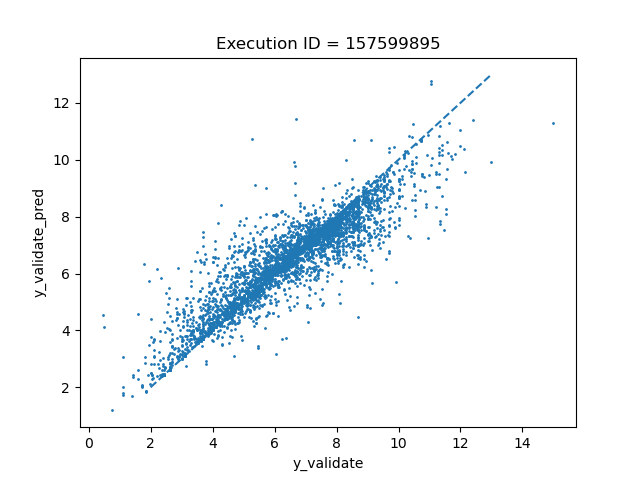
\includegraphics[width=0.40\textwidth]{images/accuracy_validate}
    \caption{(Sample) Visualizing accuracy.  $R^2 \approx 0.805$.}
    \label{fig:modelQualityVisualization}
\end{figure}

\end{frame}

\section{Machine Learning Models \& Results}
\begin{frame}[t]{Machine Learning models}
The ML model should approximate the following function:
$$ \textrm{Binding affinity prediction} : \mathbf{R}^n \mapsto \mathbf{R} \;\; \textrm{where} \;\; n \in \mathbf{I}^+$$
The following ML models were studied
\begin{itemize}
\item Simple Linear Regression
\item Random Forest Regression
\item Support Vector Regression
\item Rotation Forest Regression
\end{itemize}
Also Note:
\begin{itemize}
\item DNNs could not be used due to lack of data.  
\item The project only had $\approx 16000$ data points to train.
\item A simple DNN a model of size $[457,  20, 10,  1]$ has 9350 parameters.
\item The DNN would overfit drastically.
\end{itemize}

\end{frame}

\begin{frame}[t]{Simple Linear Regression}
\begin{itemize}
\item This model approximates the binding affinity using a linear hyperplane.  (By minimizing the square of errors).
\item It is the cheapest computational model.
\item Assumes strong linear relationship between input features and binding affinity.
\item Genetic algorithms sucessfully used for feature selection.
\item Alternate weighting strategy: Data duplication.
\end{itemize}

\begin{table} [h!]
\centering
\resizebox{0.75\linewidth}{!} {
\begin{tabular}{ | c | c | c | c | c | c | }
\hline
\textbf{No.  features} & \textbf{Feature selection} & \textbf{Weighting} & \textbf{Training} & \textbf{Validation} & \textbf{Testing} \\ [0.5 ex]
\hline \hline
457 & - & - & 0.461 & 0.415 & 0.320\\
457 &  - & Hyperbolic & 0.454 & 0.427 & 0.337\\
457 & - & Hyperbolic duplication & 0.465 & 0.416 & 0.326\\
457 & - & Linear & 0.458 & 0.419 & 0.328\\
457 & - & Linear Duplication & 0.460 & 0.428 & 0.327\\
\textbf{49} & \textbf{Genetic} & \textbf{Hyperbolic} & \textbf{$\approx$0.377} & \textbf{$\approx$0.374}  & \textbf{$\approx$0.364}\\
40 & Pearson Correlation & Hyperbolic & 0.287 & 0.278  & 0.285 \\ 
40 & Spearman Correlation & Hyperbolic & 0.289 & 0.294  & 0.290 \\ 
176 & Manual & Hyperbolic & 0.362  & 0.346  & 0.331\\ [1ex]
\hline
\end{tabular}
}
\caption{$R^2$ scores of the Linear Regression Model.}
\label {table:1}
\end{table}

\end{frame}

\begin{frame}[t]{Random Forest Regression}
\textbf{Introduction}
\begin{itemize}
\item It is a non-linear ensemble model of regression trees.  (Sampling with replacement aka Bagging is used)
\item For each tree,  the data is split recursively till a stopping criterion.  Each data subset has lesser entropy than the superset.
\item There is no need for any assumption w.r.t data.
\item Additional feature selection strategy: Genetic Elitism.
\end{itemize}
\textbf{Dealing with correlated features}
\begin{itemize}
\item The RF was forced to randomly use only 20\% of the features to determine the best (feature, value) combination for each split step.
\item The RF model does not depend on some features exclusively.
\item The correlated features were used as an advantage.
\end{itemize}
\end{frame}
 
 \begin{frame}[t]{Random Forest Regression}
\textbf{Feature Importances}
\begin{itemize}
\item \textbf{Gini Importance:} (Provided by the RF model) 
\begin{itemize}
\item The most important features are the ones that contribute the most in the reduction in entropy.
\end{itemize}  
\item \textbf{Permutation Importance:} (Model agnostic)
\begin{itemize}
\item The most important features are the ones that are most relevant for prediction accuracy.
\end{itemize}
$$\mathrm{Importance}(f) = \mathrm{Accuracy_{pred}}(X) - \mathrm{Accuracy_{pred}}(X_{f\_shuffled})$$
\end{itemize}

\textbf{Genetic feature selection}
\begin{itemize}
\item Consider a chromosome $\mathrm{ch} = [10011....1...]$
\item $\mathrm{Score}(\mathrm{ch}) = \mathrm{Importance}(f_1,  f_4, f_5 ..f_{17}... ) * \mathrm{FeaturesEliminated}$
\item Reason for using different scoring function: Fitting an RF model is expensive whereas feature importance evaluation is cheap.
\end{itemize}

\end{frame}

\begin{frame}[t]{Random Forest Regression}

\begin{figure}
     \centering
     \begin{subfigure}[b]{0.49\textwidth}
         \centering
         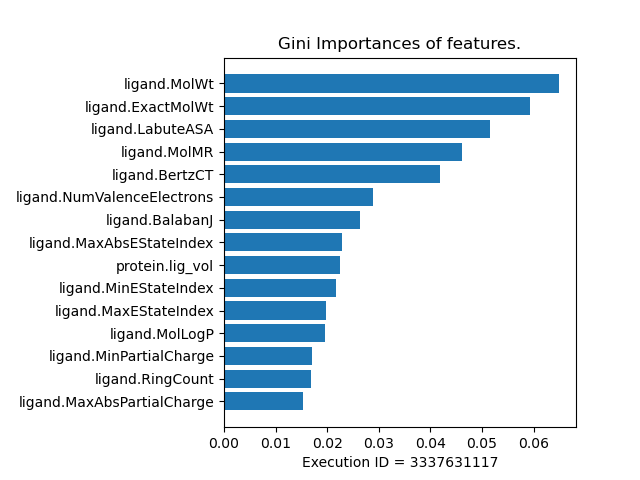
\includegraphics[scale=0.23]{images/Gini_importance}
         \caption{Gini importance.}
        \label{fig:GiniImportanceLabel}
     \end{subfigure}
     \hfill
     \begin{subfigure}[b]{0.49\textwidth}
         \centering
         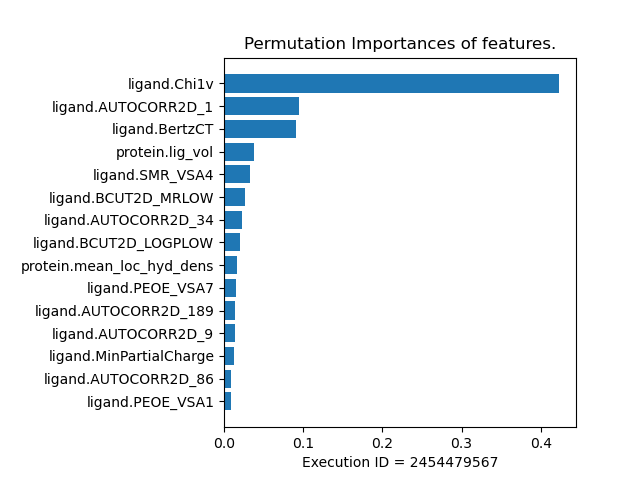
\includegraphics[scale=0.23]{images/Permutation_importance}
        \caption{Permutation importance.}
        \label{fig:PermutationImportanceLabel}
     \end{subfigure}
     \caption{Feature Importance calculation of Random Forest Regressor (With manual feature selection).}
     \label{fig:RFMFILable}
\end{figure}

\begin{table} [h!]
\centering
\resizebox{0.7\linewidth}{!} {
 \begin{tabular}{ | c | c |  c | c | c | c | c |}
\hline
\textbf{No.  Features} & \textbf{Feature Selection} & \textbf{Weighting} & \textbf{Training} & \textbf{Validation} & \textbf{OOB score} & \textbf{Testing} \\ [0.5 ex]
\hline \hline
457 & - & - & 0.961 & 0.790 & 0.791 & 0.447\\
457 & - & Hyperbolic &  0.961 & 0.773 & 0.794 & 0.448\\
457 & - & Linear &  0.960 & 0.785 & 0.794 & 0.443\\
40 & Spearman Correlation & Hyperbolic &  0.930 & 0.664 & 0.671 & 0.878  \\ 
40 & Pearson Correlation & Hyperbolic &  0.925 & 0.642 & 0.645 & 0.868  \\ 
229 & Genetic Elitism & Hyperbolic  & 0.958 &  0.779 & 0.793 & 0.444 \\
394 & Genetic Normal& Hyperbolic & 0.961 & 0.776 & 0.795 & 0.448 \\
\textbf{176} & \textbf{manual}  & \textbf{Hyperbolic} &  \textbf{0.949} & \textbf{0.734} & \textbf{0.736} & \textbf{0.463}  \\ [1ex]
\hline
\end{tabular}
}
\caption{Random Forest Regression $R^2$ Score table.}
\label {table:3}
\end{table}

\end{frame}

\begin{frame}[t]{Support Vector Regression}
\begin{itemize}
\item It is a non linear model.
\item It fits a $\epsilon$ radius pipe to the data.
\item The model was not suitable for running genetic algorithms (for both normal and permutation genetics).  Training took $\approx 99.07 s$ and validation took $\approx 27.01 s$.
\item Features were selected using either output correlation or manual feature selection.
\item Contrary to other models,  linear weighting of data gave the best results.
\end{itemize}

\begin{table} [h!]
\centering
\resizebox{0.7\linewidth}{!} {
 \begin{tabular}{ | c | c | c | c | c | c | }
\hline
\textbf{No. Features} & \textbf{Feature Selection} & \textbf{Weighting} & \textbf{Training} & \textbf{Validation} &  \textbf{Testing} \\ [0.5 ex]
\hline \hline
457 & - & - & 0.311 & 0.290 & 0.314\\
457 & - & Hyperbolic & 0.330 & 0.323 & 0.327\\
\textbf{457} & \textbf{-} & \textbf{Linear}  & \textbf{0.344} &\textbf{0.319} & \textbf{0.335}\\
40 & Spearman Correlation & Linear & 0.260 & 0.268  & 0.262 \\ 
40 & Pearson Correlation & Linear & 0.198 & 0.196 & 0.197 \\ 
40 & Spearman Correlation & Hyperbolic & 0.254 & 0.265 & 0.256 \\ 
40 & Pearson Correlation & Hyperbolic & 0.168 & 0.171 & 0.168 \\ 
176 & Manual & Linear &  0.311  & 0.283  & 0.310\\ [1ex]
\hline
\end{tabular}
}
\caption{Table showing  $R^2$ Scores for SVR.}
\label {table:2}
\end{table}

\end{frame}

\begin{frame}[t]{Rotation Forest Regression}
\begin{itemize}
\item Random forest trees divide data using axis aligned hyperplanes.
\item The complexity of the trees can be reduced by linearly transforming (rotating) the data.  The eigen vectors of the training data become the basis vectors.  For example:
\begin{itemize}
\item Representing $y = kx$ would take a very deep tree.
\item If $y = kx$ is linearly transformed to $y = 0$,  only 1 node is enough.
\end{itemize}

\item Computationally very expensive - It took $\approx$ 25 min 29 seconds to train.
\end{itemize}

\begin{table} [h!]
\centering
\resizebox{0.7\linewidth}{!} {
 \begin{tabular}{ | c | c | c | c | c | }
\hline
\textbf{No.  Features} & \textbf{Feature Selection} & \textbf{Training} & \textbf{Validation} & \textbf{Testing} \\ [0.5 ex]
\hline \hline
457 & - & 0.967 & 0.767 & 0.449\\
40 & Spearman Correlation & 0.952 & 0.650 & 0.890\\
40 & Pearson Correlation & 0.951 & 0.629 & 0.883 \\
\textbf{176} & \textbf{manual} & \textbf{0.960} & \textbf{0.716} & \textbf{0.471} \\ [1ex]
\hline
\end{tabular}
}
\caption{Rotation Forest $R^2$ Score overview.}
\label {table:4}
\end{table}

\end{frame}

\section{Discussion}
\begin{frame}[t]{Discussion}
Notable points:
\begin{itemize}
\item Best models: Linear Regression and Random Forest Regression.
\item Random Forest uses correlated features to make itself more robust.
\item Random Forest can deal with both discrete and real valued features.
\item Rotation Forest did not improvement accuracy as they are good only for Real valued features.
\item Testing results were sometimes better than validation results. It is because test data $<$ validation data.
But the difference is minimal.
\end{itemize} 
Limitations:
\begin{itemize}
\item Linear regression assumes data linearity.
\item Random Forest has heavy reliance on ligand features.
\item Both models were black box models.
\item Genetic feature selection was not helpful for Random Forests.

\end{itemize} 
\end{frame}

\begin{frame}[t]{Discussion}
Further work:
\begin{itemize}
\item A new weighting strategy: Weighting a pocket descriptor based on the overlap between the pocket and the ligand.  For example,
$$
W_\mathrm{Total} = W_\mathrm{Hyperbolic} * W_\mathrm{Overlap}
$$
\item Improvement of feature selection: Build 1 model per family of features. Use the best feature as a family surrogate.
\item A more explainable model can be built.
\end{itemize} 

\end{frame}

\section{Q \& A}

\begin{frame}[t]{Q \& A}
  \centering \Huge
  \emph{Q \& A}
\end{frame}

\section{References}

\begin{frame}[t]{References}

\begin{thebibliography}{1}

\bibitem{proteinlingandbindingpaper}
\alert{Du,  Li,  Xia,  Ai,  Liang,  Sang,  Ji and Liu; Insights into Protein–Ligand Interactions: Mechanisms, Models, and Methods (2016)}

\bibitem{fpocketpaper}
\alert{Le Guilloux,  Schmidtke, and Tuffery; Fpocket: An open source platform for ligand pocket detection(2009)}

\bibitem{drugdiscoverycost}
\alert{DiMasi,  Grabowski and Hansen; nnovation in the pharmaceutical industry: New estimates of R \& D costs (2016)}

\bibitem{geneticalgorithmsresearchpaper}
\alert{John H. Holland.  Genetic Algorithms. (1960)}

\bibitem{bagnall2020rotation}
\alert{Is rotation forest the best classifier for problems with continuous features? A. Bagnall, M. Flynn, J. Large, J. Line, A. Bostrom, and G. Cawley (2020)}

\end{thebibliography}

\end{frame}

\section{Appendix}

\begin{frame}[t]{Appendix - Definitions}

\begin{itemize}
\item Binding affinity between a protein and a ligand is quantified by the $K_d$, $K_i$ and $IC_{50}$.
Here $K_d$ refers to the dissociation constant, $K_i$ to inhibition constant, and $IC_{50}$ to 
inhibitory concentration 50\%.
\end{itemize}
\end{frame}

\begin{frame}[t]{Appendix - Feature Extraction}
\textbf{Protein Features:}
\begin{itemize}
\item \textit{fpocket} is an LBS prediction algorithm used to predict ligand binding pockets.
\item There can be multiple binding pockets for a PL complex.
\item Using \textit{dpocket},  $55$ descriptors were obtained for every (potentially) binding pocket as real values.
\end{itemize}

\textbf{Ligand Features:}
\begin{itemize}
\item Using \textit{RDKit.Chem.Descriptors} module,  $402$ features were extracted as real values.
\end{itemize}

\textbf{Concatenation:}
\begin{itemize}
\item The (concatenated) input feature space to the model was $\mathbf{R}^{457}$.
\item It was less than $\mathbf{R}^{457}$ if feature selection is done before model training.
\end{itemize}

\end{frame}


\begin{frame}[t]{Appendix - Visualizing Linear Regression results}
\begin{figure}
     \centering
     \begin{subfigure}[b]{0.45\textwidth}
         \centering
         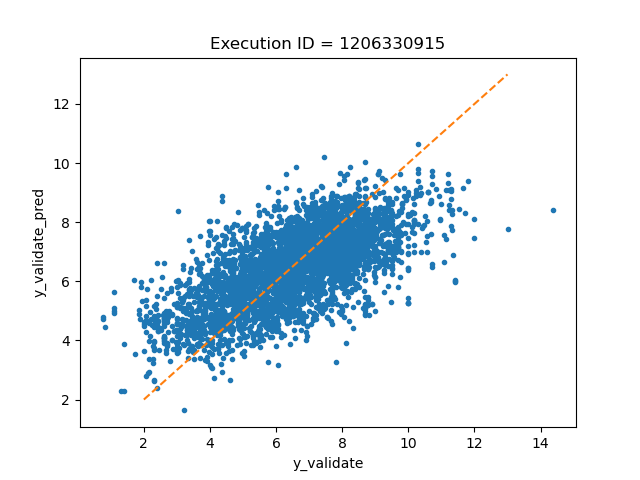
\includegraphics[scale=0.35]{images/accuracyValidateLGHyperbolic}
         \caption{Validation accuracy.}
        \label{fig:accuracyValidateLGHyperbolic}
     \end{subfigure}
     \hfill
     \begin{subfigure}[b]{0.45\textwidth}
         \centering
         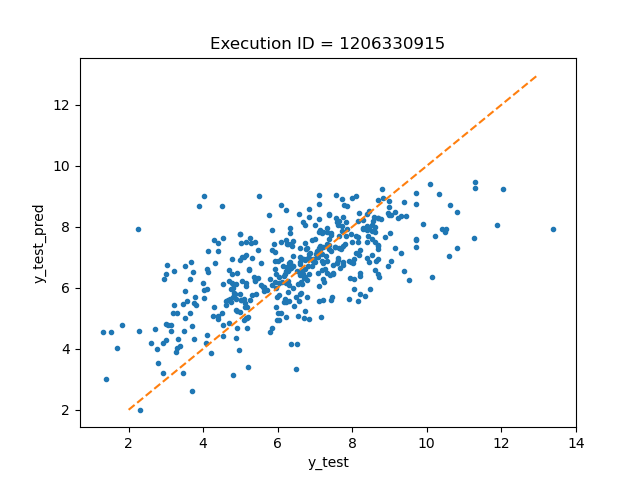
\includegraphics[scale=0.35]{images/accuracytestLGHyperbolic}
        \caption{Testing accuracy.}
        \label{fig:accuracytestLGHyperbolic}
     \end{subfigure}
     \caption{Linear Model using Hyperbolic weighting and all 49 features selected by genetic algorithm.}
     \label{fig:BestLinearModel}
\end{figure}
\end{frame}

\begin{frame}[t]{Appendix - Visualizing Random Forest results}
\begin{figure}
     \centering
     \begin{subfigure}[b]{0.45\textwidth}
         \centering
         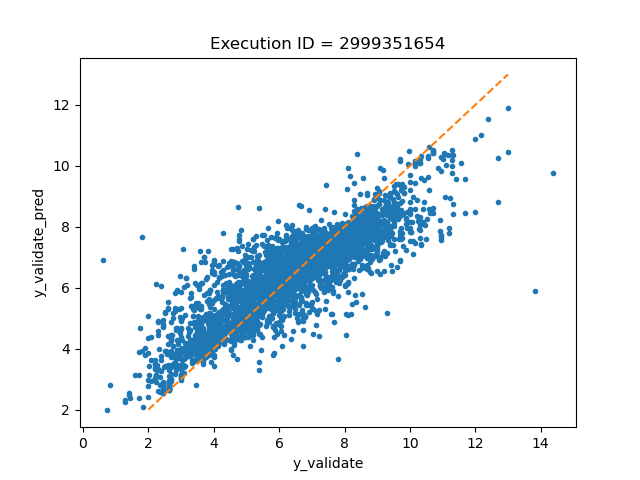
\includegraphics[scale=0.35]{images/accuracyRFRvalidate}
         \caption{Validation accuracy.}
        \label{fig:accuracyRFRvalidate}
     \end{subfigure}
     \hfill
     \begin{subfigure}[b]{0.45\textwidth}
         \centering
         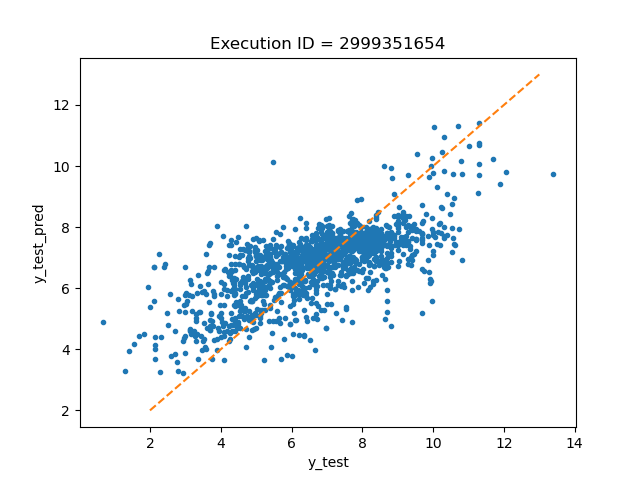
\includegraphics[scale=0.35]{images/accuracyRFRtest}
        \caption{Testing accuracy.}
        \label{fig:accuracyRFRtest}
     \end{subfigure}
     \caption{Random Forest Regressor with 176 manually selected features and hyperbolic weighting.}
     \label{fig:RFMModel}
\end{figure}
\end{frame}


\begin{frame}[t]{Appendix - Visualizing SVR Results}
\begin{figure}
     \centering
     \begin{subfigure}[b]{0.45\textwidth}
         \centering
         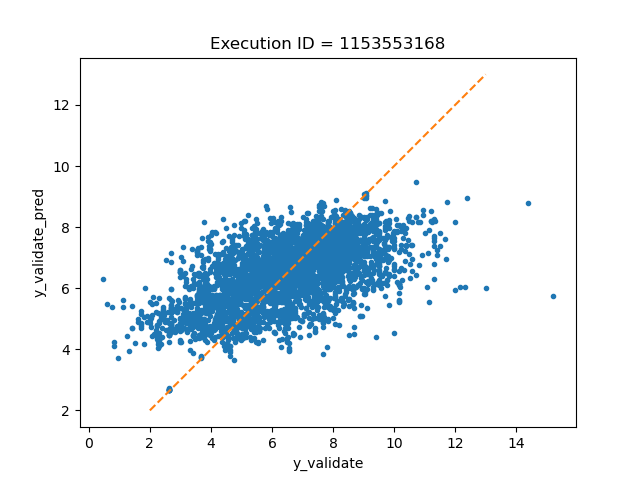
\includegraphics[scale=0.35]{images/SVRvalidate}
         \caption{Validation accuracy.}
        \label{fig:SVRvalidate}
     \end{subfigure}
     \hfill
     \begin{subfigure}[b]{0.45\textwidth}
         \centering
         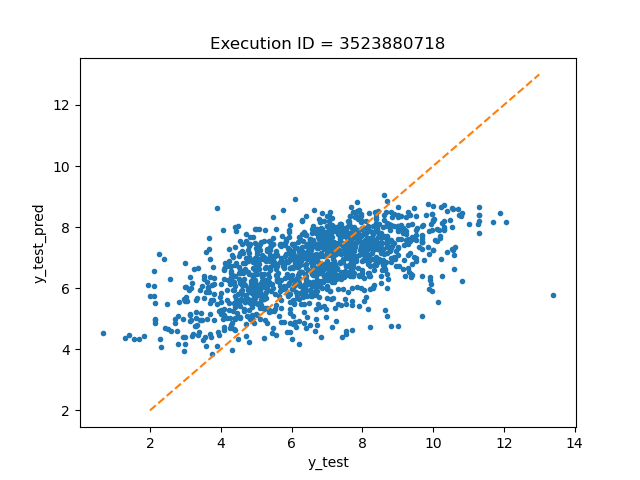
\includegraphics[scale=0.35]{images/SVRtest}
        \caption{Testing accuracy.}
        \label{fig:SVRtest}
     \end{subfigure}
     \caption{SVR accuracy visualization for all features 457 and Linear weighting.}
     \label{fig:SVRaccuracy}
\end{figure}
\end{frame}

\begin{frame}[t]{Appendix - Visualizing Rotation Forest Results}
\begin{figure}
     \centering
     \begin{subfigure}[b]{0.45\textwidth}
         \centering
         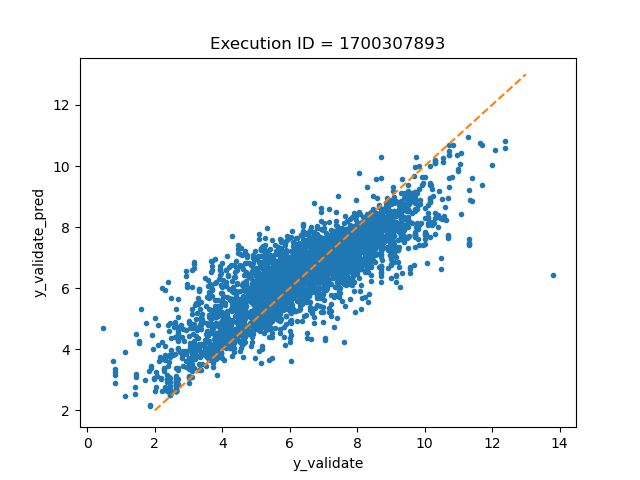
\includegraphics[scale=0.35]{images/accuracyRotationFRvalidate}
         \caption{Validation accuracy.}
        \label{fig:accuracyRotationFRvalidate}
     \end{subfigure}
     \hfill
     \begin{subfigure}[b]{0.45\textwidth}
         \centering
         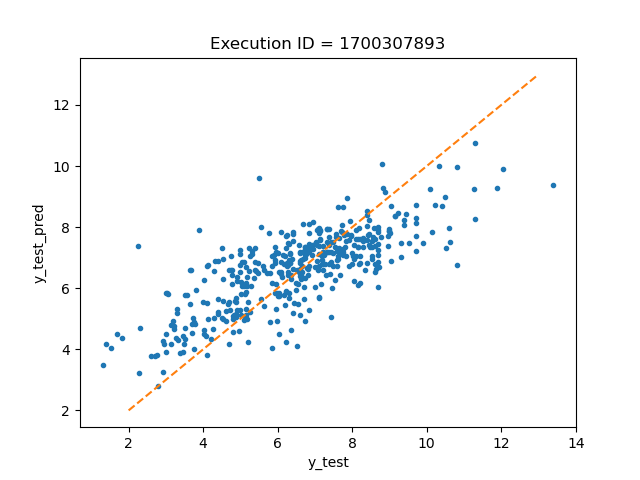
\includegraphics[scale=0.35]{images/accuracyRotationFRtest}
        \caption{Testing accuracy.}
        \label{fig:accuracyRotationFRtest}
     \end{subfigure}
     \caption{Rotation Forest Accuracy visualization for manually selected features (176).  The rotation forest implementation does not support data weighting.}
     \label{fig:RotationForestAccuracy}
\end{figure}
\end{frame}

\end{document}
